% Apresentações em widescreen. Outros valores possíveis: 1610, 149, 54, 43 e 32.
% Por padrão, as apresentações são no formato 4:3 (sem o aspectratio).
\documentclass[aspectratio=169]{beamer}	 	

\usetheme{Berkeley}
\usecolortheme{default}
\usefonttheme[onlymath]{serif}			% para fontes matemáticas

% ---
% PACOTES
% --
\usepackage[alf]{abntex2cite}		% Citações padrão ABNT
\usepackage[brazil]{babel}		    % Idioma do documento
\usepackage{color}			       % Controle das cores
\usepackage[T1]{fontenc}		  % Selecao de codigos de fonte.
\usepackage{graphicx}			    % Inclusão de gráficos
\usepackage[utf8]{inputenc}		   % Codificacao do documento (conversão automática dos acentos)
\usepackage{multirow}
\usepackage{threeparttable}
\usepackage[capposition=top]{floatrow}
\usepackage{txfonts}			 % Fontes virtuais
\usepackage{ragged2e}
\usepackage{etoolbox}
\usepackage{lipsum}
% ---

% ---
% Minhas Definições
% ---

%Deixando o Caption alinhado a esquerda mesmo com quebra de linha
\usepackage[labelfont=bf, justification=justified,singlelinecheck=true]{caption}

%Justificando o corpo do texto
\renewcommand{\raggedright}{\leftskip=0pt \rightskip=0pt plus 0cm} 

% Colocando numero de paginas no slide
\setbeamertemplate{footline}[frame number]
\setbeamertemplate{caption}[numbered]
% Tela cheia
%\hypersetup{pdfpagemode=FullScreen}
% ---


% --- Informações do documento ---
\logo{
\includegraphics[scale=0.15]{figuras/logo.png}}
\title{Ambiente Virtual de Aprendizagem para Auxiliar no Processo de Ensino e Aprendizagem de Matemática}
\author{Marciano Machado Saraiva}
\institute{
Orientador: Prof. Me. Samy Soares Passos de Sá\\[2 ex]
Universidade Federal do Ceará
	    \par
	    Bacharel em Sistemas de Informação}
\date{\today}
% ---

% ----------------- INÍCIO DO DOCUMENTO --------------------------------------
\begin{document}

% ----------------- NOVO SLIDE --------------------------------
\begin{frame}

    \titlepage

\end{frame}

% ----------------- NOVO SLIDE --------------------------------
\begin{frame}{Roteiro}
	\tableofcontents
\end{frame}

%% ----------------- NOVO SLIDE --------------------------------
\section{Introdução}

\begin{frame}{Introdução}
\framesubtitle{Motivação}

\begin{itemize}
	\item Grande número de reprovações e desistências em turmas iniciais de Matemática de cursos na Universidade Federal do Ceará - Campus Quixadá.
	\item A Organização para Cooperação e Desenvolvimento Econômico(OECD) revelou que em 2015, 67.1\% do alunos estavam abaixo do nível 2 (os níveis vão de 1 a 6) na escala do PISA \cite{pisainfocus2016}.

\end{itemize}

\end{frame}

% ----------------- NOVO SLIDE --------------------------------
\begin{frame}
\frametitle{Introdução}
\framesubtitle{Objetivos}

\begin{block}{Objetivo Geral}
	Desenvolver um Ambiente Virtual de Aprendizagem para auxiliar no processo de ensino e aprendizagem de matemática por alunos dentro e fora da sala de aula.
\end{block}

\begin{block}{Objetivos Específicos}
  \begin{itemize}
  \item Levantar os requisitos do sistema.
  \pause
  \item Desenvolver os módulos com funções de administração do sistema.
  \pause
  \item Desenvolver os módulos com funções que serão utilizadas pelos estudantes aplicando técnicas de Gamificação.
  \pause
  \item Verificar a influência e impactos provocados pelo AVA no aprendizado de alunos por meio de exames aplicados a cada estudante antes e após o uso do sistema na Universidade Federal do Ceará.
\end{itemize}
\end{block}

\end{frame}

% ----------------- NOVO SLIDE --------------------------------
\section{Revisão Bibliográfica}

\begin{frame}{Revisão Bibliográfica}
  \begin{itemize}
  	\item Metodologias no Ensino da Matemática
    	\begin{itemize}
        	\item Aula Expositiva
            \item Resolução de Problemas
            \item Modelagem Matemática
            \item O uso de computadores
        \end{itemize}
    \item Ambientes Virtuais de Aprendizagem
    \item Gamificação 
  \end{itemize}
\end{frame}

% ----------------- NOVO SLIDE --------------------------------
\begin{frame}{Trabalhos Relacionados}
\frametitle{Revisão Bibliográfica}
\framesubtitle{Trabalhos Relacionados}

\begin{itemize}
	\item The one world schoolhouse: Education reimagined.
    \item ActiveMath: A generic and adaptive web-based learning environment.
    \item Duolingo: Learn a Language for Free while Helping to Translate the Web.
    \item Resolução de problemas em ambientes virtuais de aprendizagem num curso de licenciatura em matemática na modalidade a distância.
\end{itemize}

\end{frame}

% ----------------- NOVO SLIDE --------------------------------
\section{Descrição da Proposta}

\begin{frame}{Descrição da Proposta}

\begin{overprint}

\only<1>{
	\begin{figure}[H]
	\centering
	\caption{Representa\c{c}\~ao }
	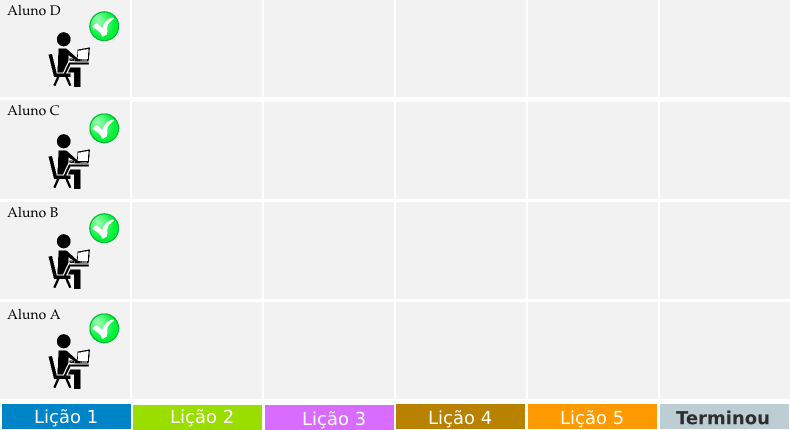
\includegraphics[width=10cm]{figuras/proposta/imagem1.png}
	\floatfoot{Fonte: Elaborada pelo autor}
	\end{figure}
}
\only<2>{
	\begin{figure}[H]
	\centering
	\caption{Turmas}
	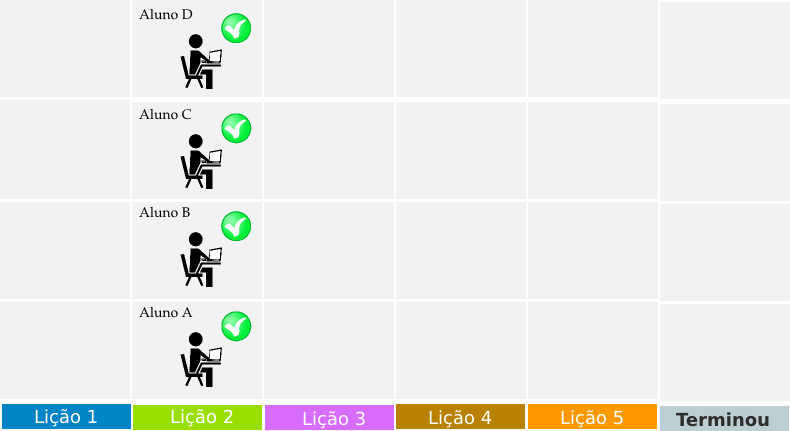
\includegraphics[width=10cm]{figuras/proposta/imagem2.png}
	\floatfoot{Fonte: Elaborada pelo autor}
	\end{figure}
}
\only<3>{
	\begin{figure}[H]
	\centering
	\caption{Turmas}
	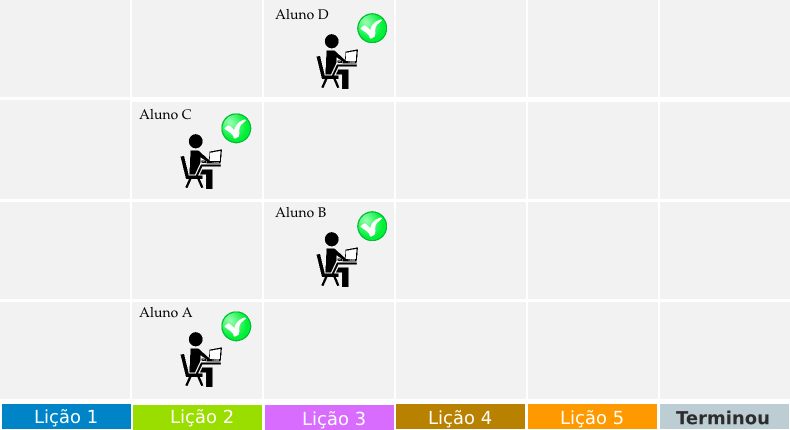
\includegraphics[width=10cm]{figuras/proposta/imagem3.png}
	\floatfoot{Fonte: Elaborada pelo autor}
	\end{figure}
}
\only<4>{
	\begin{figure}[H]
	\centering
	\caption{Turmas}
	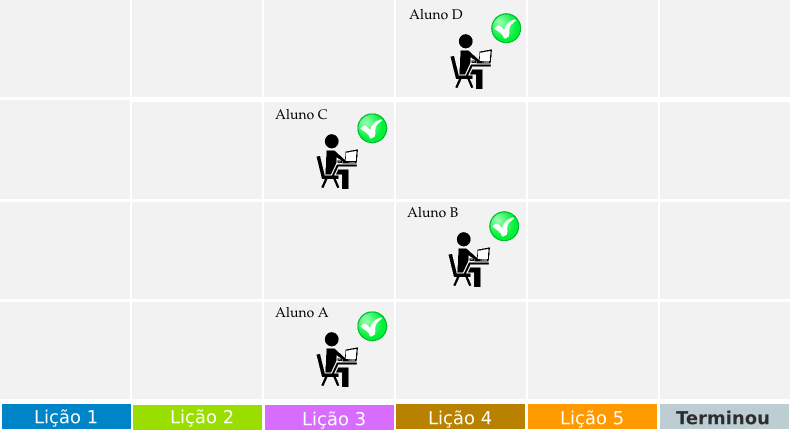
\includegraphics[width=10cm]{figuras/proposta/imagem4.png}
	\floatfoot{Fonte: Elaborada pelo autor}
	\end{figure}
}
\only<5>{
	\begin{figure}[H]
	\centering
	\caption{Turmas}
	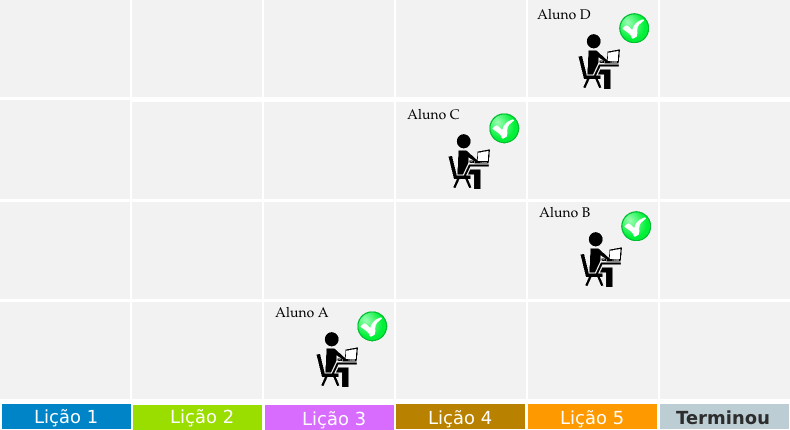
\includegraphics[width=10cm]{figuras/proposta/imagem5.png}
	\floatfoot{Fonte: Elaborada pelo autor}
	\end{figure}
}
\only<6>{
	\begin{figure}[H]
	\centering
	\caption{Turmas}
	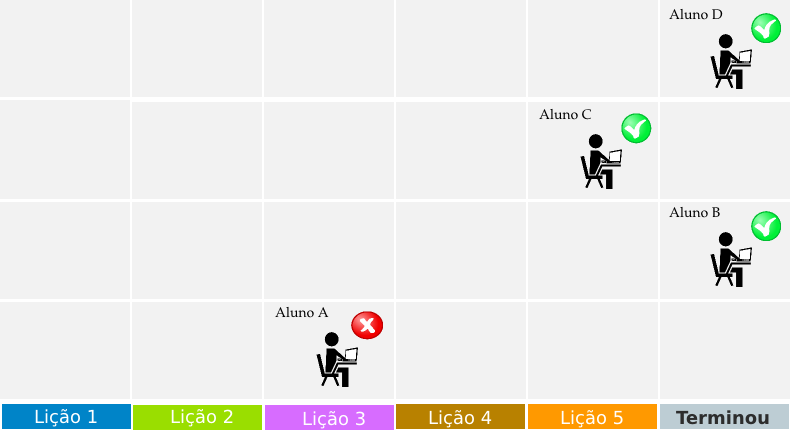
\includegraphics[width=10cm]{figuras/proposta/imagem6.png}
	\floatfoot{Fonte: Elaborada pelo autor}
	\end{figure}
}
\only<7>{
	\begin{figure}[H]
	\centering
	\caption{Turmas}
	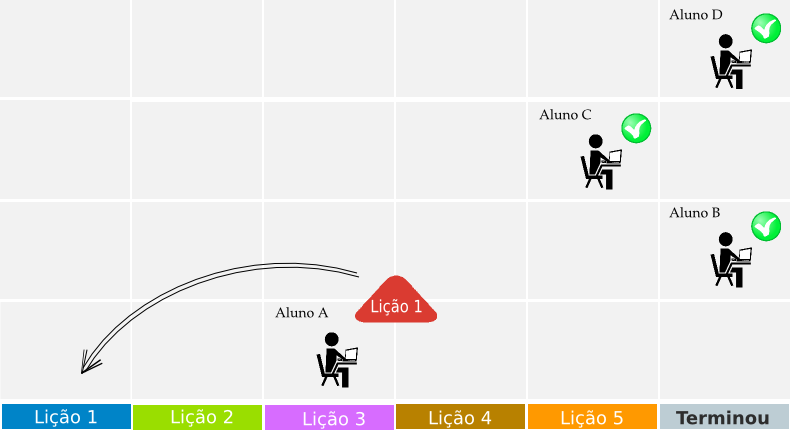
\includegraphics[width=10cm]{figuras/proposta/imagem7.png}
	\floatfoot{Fonte: Elaborada pelo autor}
	\end{figure}
}
\only<8>{
	\begin{figure}[H]
	\centering
	\caption{Turmas}
	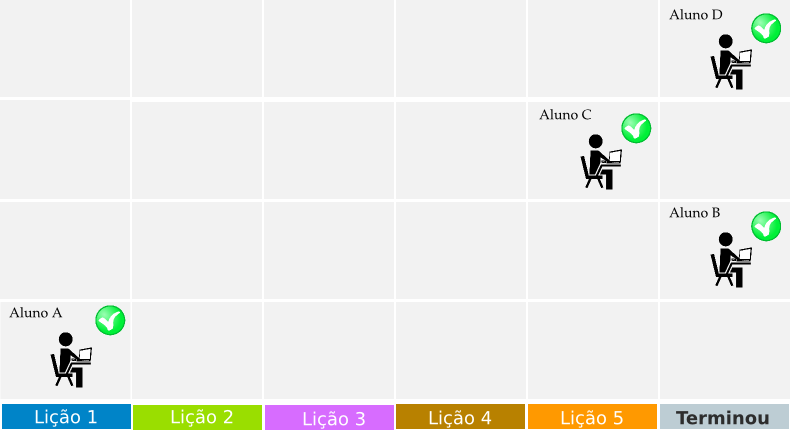
\includegraphics[width=10cm]{figuras/proposta/imagem8.png}
	\floatfoot{Fonte: Elaborada pelo autor}
	\end{figure}
}
\only<9>{
	\begin{figure}[H]
	\centering
	\caption{Turmas}
	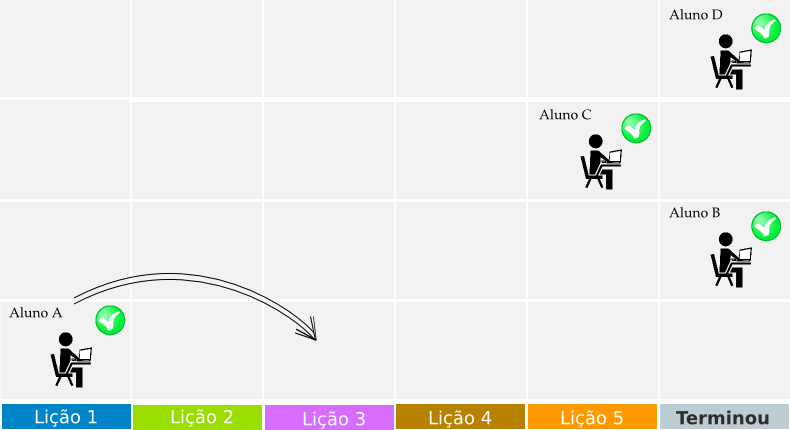
\includegraphics[width=10cm]{figuras/proposta/imagem9.png}
	\floatfoot{Fonte: Elaborada pelo autor}
	\end{figure}
}
\only<10>{
	\begin{figure}[H]
	\centering
	\caption{Turmas}
	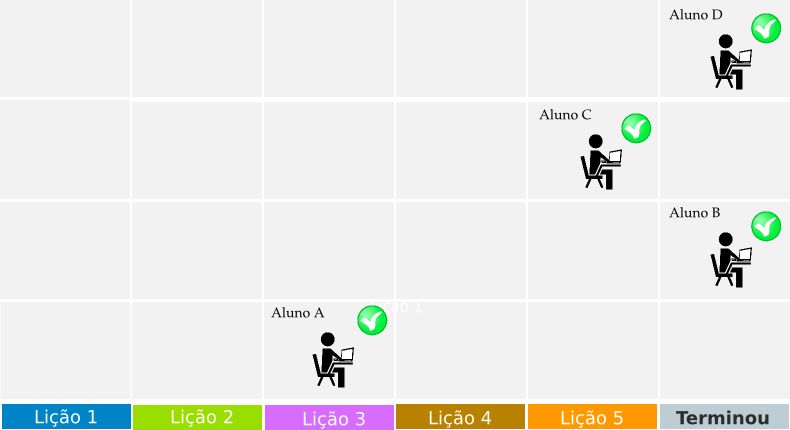
\includegraphics[width=10cm]{figuras/proposta/imagem10.png}
	\floatfoot{Fonte: Elaborada pelo autor}
	\end{figure}
}

\end{overprint}

\end{frame}

% ----------------- NOVO SLIDE --------------------------------
\section{Procedimentos Metodológicos}

\begin{frame}{Procedimentos Metodológicos}
	\begin{enumerate}
    	\item Definição do Processo
        \item Levantamento e Análise de Requisitos
        \item Projeto do Sistema
        \item Implementação do Sistema
        \item Verificação e Validação
        \item Definição do Conteúdo para o Sistema
        \item Aplicação da Solução na Universidade Federal do Ceará - Campus Quixadá
    \end{enumerate}
\end{frame}

% ----------------- NOVO SLIDE --------------------------------

\begin{frame}{Procedimentos Metodológicos}
\frametitle{Procedimentos Metodológicos}
\framesubtitle{Definição do Processo}

\citeonline{padua2003engenharia} descreve um processo como um conjunto de passos parcialmente ordenados, constituídos por atividades, métodos, práticas e transformações, usados para atingir uma meta.

\end{frame}

% ----------------- NOVO SLIDE --------------------------------

\begin{frame}{Procedimentos Metodológicos}
\frametitle{Procedimentos Metodológicos}
\framesubtitle{Levantamento e Análise de Requisitos}

O Levantamento e Análise de Requisitos é a fase em que verificamos quais as necessidades, condições e princípios que o software deverá atender \cite{matuda2013mapas}.
\pause
\begin{enumerate}
	\item Definimos o público-alvo e criamos Personas.
    \pause
	\item Coletamos os requisitos através de entrevistas semi-estruturadas.
    \pause
    \item Realizamos a análise dos requisitos.
    \pause
    \item Desenvolvemos uma documentação para os requisitos.
\end{enumerate}

\end{frame}

% ----------------- NOVO SLIDE --------------------------------

\begin{frame}{Procedimentos Metodológicos}
\frametitle{Procedimentos Metodológicos}
\framesubtitle{Projeto do Sistema}

O Projeto de Software é à atividade de engenharia cujo foco é definir ``como'' os requisitos estabelecidos no projeto devem ser implementados no software \cite{pressman2006engenharia}.
\pause
\begin{enumerate}
	\item Definimos a Arquitetura do sistema.
    \item Escolhemos as ferramentas utilizadas.
\end{enumerate}
\end{frame}

% ----------------- NOVO SLIDE --------------------------------

\begin{frame}{Procedimentos Metodológicos}
\frametitle{Procedimentos Metodológicos}
\framesubtitle{Implementação do Sistema}

A implementação envolve as atividades de codificação, compilação e integração.
\begin{block}{Ambiente de Desenvolvimento}
	 \begin{itemize}
	  \item \textbf{Sistema Operacional}: Ubuntu 14.04 LTS;
	  \item \textbf{Interpretador}: Python 2.7.6;
	  \item \textbf{Banco de Dados}: PostgreSQL 9.3.13;
	  \item \textbf{Framework de back-end}: DJango 1.7.11;
	  \item \textbf{Framework de front-end}: Metro UI CSS 3.0.15;
	  \item \textbf{Virtualiza\c{c}\~ao}: Virtualenv 15.0.2;
	  \item \textbf{Controle de Vers\~ao}: Git 1.9.1;
	 \end{itemize}

\end{block}


\end{frame}

% ----------------- NOVO SLIDE --------------------------------

\begin{frame}{Procedimentos Metodológicos}
\frametitle{Procedimentos Metodológicos}
\framesubtitle{Verificação e Validação}

Essa etapa deve mostrar que o sistema está de acordo com a especificação e que ele atende às expectativas de clientes e usuários, além de assegurar que o programa está fazendo aquilo que foi definido 
em sua especificação e que não possui erros de execução \cite{aguiar2012requisitos}.

\begin{block}{Testes que ser\~ao realizados}
	\begin{itemize}
	 \item \textbf{Teste de Unidade} – é aquele que testa uma única unidade do sistema.
	 \item \textbf{Teste de Integração} – é aquele que testa a integração entre duas ou mais partes de um sistema.
	 \item \textbf{Teste de Sistema} – é aquele que garante que o sistema funciona como um todo.
	\end{itemize}

\end{block}


\end{frame}

% ----------------- NOVO SLIDE --------------------------------

\begin{frame}{Procedimentos Metodológicos}
\frametitle{Procedimentos Metodológicos}
\framesubtitle{Definição do Conteúdo para o Sistema}
	\begin{itemize}
	 \item A aplicação da primeira versão do sistema ocorrer\'a em duas turmas de Matemática na Universidade
Federal do Ceará - Campus Quixadá.
	\item Os monitores dessas turmas passaram por um treinamento, em que aprender\~ao a utilizar o sistema para assim, adicionarem os conte\'udos.
	\end{itemize}

\end{frame}

% ----------------- NOVO SLIDE --------------------------------

\begin{frame}{Procedimentos Metodológicos}
\frametitle{Procedimentos Metodológicos}
\framesubtitle{Aplicação da Solução na Universidade Federal do Ceará - Campus Quixadá}

\begin{figure}[H]
\centering
\caption{Turmas}
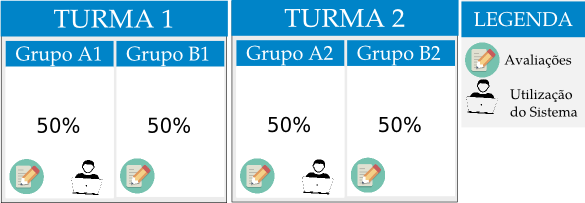
\includegraphics[width=10cm]{figuras/aplicacao.png}
\label{figura_aplicacao}
\floatfoot{Fonte: Elaborada pelo autor}
\end{figure}

\end{frame}

% ----------------- NOVO SLIDE --------------------------------

\begin{frame}{Procedimentos Metodológicos}
\frametitle{Procedimentos Metodológicos}
\framesubtitle{Cronograma}
	\begin{table}[H]
\centering
\caption{Cronograma de Execução}
\label{cronograma}

\resizebox{\textwidth}{!}{
\begin{tabular}{|l|c|c|c|c|c|c|c|c|c|c|c|c|c|c|c|}
\hline
\multicolumn{1}{|c|}{\multirow{2}{*}{ATIVIDADES}} & \multicolumn{6}{c|}{2015} & \multicolumn{9}{c|}{2016} \\ \cline{2-16} 
\multicolumn{1}{|c|}{} & Jan & Fev & Mar & Abr & Mai & Jun - Dez & \multicolumn{1}{l|}{Jan - Mar} & \multicolumn{1}{l|}{Abr} & \multicolumn{1}{l|}{Mai} & \multicolumn{1}{l|}{Jun} & \multicolumn{1}{l|}{Jul} & \multicolumn{1}{l|}{Ago} & \multicolumn{1}{l|}{Set} & \multicolumn{1}{l|}{Out} & \multicolumn{1}{l|}{Nov} \\ \hline
Definição do Processo & x &  &  &  &  &  &  &  &  &  &  &  &  &  &  \\ \hline
Levantamento e Análise dos Requisitos & x & x & x &  &  &  &  &  &  &  &  &  &  &  &  \\ \hline
Projeto do Sistema &  &  &  & x & x &  &  &  &  &  &  &  &  &  &  \\ \hline
Implementação do Sistema &  &  &  &  &  & x & x & x & x & x &  &  &  &  &  \\ \hline
Verificação e Validação &  &  &  &  &  &  &  &  &  &  & x &  &  &  &  \\ \hline
Desenvolver o conteúdo para o sistema &  &  &  &  &  &  &  & x & x & x & x & x &  &  &  \\ \hline
Aplicação na UFC - Campus Quixadá &  &  &  &  &  &  &  &  &  &  &  & x & x & x &  \\ \hline
Definição do Projeto de Pesquisa &  &  &  &  &  &  &  & x &  &  &  &  &  &  &  \\ \hline
Defesa do Projeto de Pesquisa &  &  &  &  &  &  &  &  &  & x &  &  &  &  &  \\ \hline
Ajustes Solicitados &  &  &  &  &  &  &  &  &  &  & x &  &  &  &  \\ \hline
Análise dos Resultados Obtidos na Aplicação. &  &  &  &  &  &  &  &  &  &  &  &  &  &  & x \\ \hline
Defesa do Trabalho Final &  &  &  &  &  &  &  &  &  &  &  &  &  &  & x \\ \hline
\end{tabular}}
\fnote{Fonte: Elaborado pelo autor}
\end{table}
\end{frame}


% ----------------- NOVO SLIDE --------------------------------
\section{Resultados Preliminares}
\begin{frame}{Resultados Preliminares}

\begin{overprint}

\only<1>{
	\begin{enumerate}
    	\item Definição do Processo 
\includegraphics[width=0.03\textwidth]{figuras/ok}
        \item Levantamento e Análise de Requisitos 
\includegraphics[width=0.03\textwidth]{figuras/ok}
        \item Projeto do Sistema 
\includegraphics[width=0.03\textwidth]{figuras/ok}
        \item Implementação do Sistema 
\includegraphics[width=0.03\textwidth]{figuras/deploy}
        \item Verificação e Validação
        \item Definição do Conteúdo para o Sistema 
\includegraphics[width=0.03\textwidth]{figuras/deploy}
        \item Aplicação da Solução na Universidade Federal do Ceará - Campus Quixadá
    \end{enumerate}
}

\only<2>{
Etapa de Implementação:
	\begin{columns}[t]
		\begin{column}{.425\textwidth}
			\begin{block}{Módulos Conclu\'idos}
				\begin{itemize}
					\item Gerenciador de Usuários
					\item Gerenciador de Turmas
					\item Gerenciador de Disciplinas
					\item Gerenciador de Lições
					\item Gerenciador de Problemas
					\item Gerenciador de Pontuação
					\item F\'orum
				\end{itemize}
			\end{block}
		\end{column}
		\begin{column}{.425\textwidth}  %%<--- here
			\begin{block}{Módulos em Desenvolvimento}
				\begin{itemize}
					\item Gerenciador de Progresso
					\item Gerador de Estatísticas
					\item Ranking
				\end{itemize}
			\end{block}
		\end{column}
	\end{columns}
}

\end{overprint}

\end{frame}

% ----------------- NOVO SLIDE --------------------------------
\section{Referências}

\begin{frame}{Referências}
	\bibliography{referencias}
\end{frame}


% ----------------- FIM DO DOCUMENTO -----------------------------------------
\end{document}